%%%%%%%%%%%%%%%%%%%%%%%%%%%%%%%%%%%%%%%%%
% Beamer Presentation
% LaTeX Template
% Version 1.0 (10/11/12)
%
% This template has been downloaded from:
% http://www.LaTeXTemplates.com
%
% License:
% CC BY-NC-SA 3.0 (http://creativecommons.org/licenses/by-nc-sa/3.0/)
%
%%%%%%%%%%%%%%%%%%%%%%%%%%%%%%%%%%%%%%%%%

%----------------------------------------------------------------------------------------
%	PACKAGES AND THEMES
%----------------------------------------------------------------------------------------

\documentclass{beamer}

\mode<presentation> {

% The Beamer class comes with a number of default slide themes
% which change the colors and layouts of slides. Below this is a list
% of all the themes, uncomment each in turn to see what they look like.

%\usetheme{default}
%\usetheme{AnnArbor}
%\usetheme{Antibes}
%\usetheme{Bergen}
%\usetheme{Berkeley}
%\usetheme{Berlin}
%\usetheme{Boadilla}
%\usetheme{CambridgeUS}
%\usetheme{Copenhagen}
%\usetheme{Darmstadt}
%\usetheme{Dresden}
%\usetheme{Frankfurt}
%\usetheme{Goettingen}
%\usetheme{Hannover}
%\usetheme{Ilmenau}
%\usetheme{JuanLesPins}
%\usetheme{Luebeck}
\usetheme{Madrid}
%\usetheme{Malmoe}
%\usetheme{Marburg}
%\usetheme{Montpellier}
%\usetheme{PaloAlto}
%\usetheme{Pittsburgh}
%\usetheme{Rochester}
%\usetheme{Singapore}
%\usetheme{Szeged}
%\usetheme{Warsaw}

% As well as themes, the Beamer class has a number of color themes
% for any slide theme. Uncomment each of these in turn to see how it
% changes the colors of your current slide theme.

%\usecolortheme{albatross}
%\usecolortheme{beaver}
%\usecolortheme{beetle}
%\usecolortheme{crane}
%\usecolortheme{dolphin}
%\usecolortheme{dove}
%\usecolortheme{fly}
%\usecolortheme{lily}
%\usecolortheme{orchid}
%\usecolortheme{rose}
%\usecolortheme{seagull}
%\usecolortheme{seahorse}
%\usecolortheme{whale}
%\usecolortheme{wolverine}

%\setbeamertemplate{footline} % To remove the footer line in all slides uncomment this line
%\setbeamertemplate{footline}[page number] % To replace the footer line in all slides with a simple slide count uncomment this line

%\setbeamertemplate{navigation symbols}{} % To remove the navigation symbols from the bottom of all slides uncomment this line
}
\usepackage{hyperref}
\usepackage{graphicx} % Allows including images
\usepackage{booktabs} % Allows the use of \toprule, \midrule and \bottomrule in tables

%----------------------------------------------------------------------------------------
%	TITLE PAGE
%----------------------------------------------------------------------------------------

\title[FFT]{Fast Fourier Transform} % The short title appears at the bottom of every slide, the full title is only on the title page

\author{REZA} % Your name
\institute[UNH] % Your institution as it will appear on the bottom of every slide, may be shorthand to save space
{
University of New Hamshire \\ % Your institution for the title page
\medskip
%\textit{john@smith.com} % Your email address
}
\date{\today} % Date, can be changed to a custom date

\begin{document}
\setbeamertemplate{caption}{\raggedright\insertcaption\par}

\begin{frame}
\titlepage % Print the title page as the first slide
\end{frame}

%\begin{frame}
%\frametitle{Overview} % Table of contents slide, comment this block out to remove it
%\tableofcontents % Throughout your presentation, if you choose to use \section{} and \subsection{} commands, these will automatically be printed on this slide as an overview of your presentation
%\end{frame}

%----------------------------------------------------------------------------------------
%	PRESENTATION SLIDES
%----------------------------------------------------------------------------------------

%------------------------------------------------
\section{First Section} % Sections can be created in order to organize your presentation into discrete blocks, all sections and subsections are automatically printed in the table of contents as an overview of the talk
%------------------------------------------------

\subsection{Subsection Example} % A subsection can be created just before a set of slides with a common theme to further break down your presentation into chunks

\begin{frame}
\frametitle{What Is An FFT?}
\begin{itemize}
\item FFT stands for Fast Fourier Transform
\item FFT is an algorithm to compute the DFT of a sequnce. 
\item Fast Fourier Transforms are widely used in engineering, science, and mathematics
\end{itemize}
\end{frame}

%------------------------------------------------

%\begin{frame}
%\frametitle{DFT}

%\end{frame}

%------------------------------------------------

\begin{frame}
\frametitle{DFT}
\begin{block}{Fourier Series}
$$x_n = \frac{1}{N}\sum_{k=0}^{N-1}X_k\cdot e^{2\pi ikn/N} \ \ \ n\in\mathbb{Z}$$
\end{block}

\begin{block}{Discrete Fourier Transform}
$$X_k = \sum_{n=0}^{N-1}x_n\cdot e^{-2\pi ikn/N} \ \ \ k\in\mathbb{Z}$$
\end{block}

\end{frame}

%------------------------------------------------

%\begin{frame}
%\frametitle{Multiple Columns}
%\begin{columns}[c] % The "c" option specifies centered vertical alignment while the "t" option is used for top vertical alignment

%\column{.45\textwidth} % Left column and width
%\textbf{Heading}
%\begin{enumerate}
%\item Statement
%\item Explanation
%\item Example
%\end{enumerate}

%\column{.5\textwidth} % Right column and width
%Lorem ipsum dolor sit amet, consectetur adipiscing elit. Integer lectus nisl, ultricies in feugiat rutrum, porttitor sit amet augue. Aliquam ut tortor mauris. Sed volutpat ante purus, quis accumsan dolor.

%\end{columns}
%\end{frame}

%------------------------------------------------
\section{Second Section}
%------------------------------------------------

%\begin{frame}
%\frametitle{Table}
%\begin{table}
%\begin{tabular}{l l l}
%\toprule
%\textbf{Treatments} & \textbf{Response 1} & \textbf{Response 2}\\
%\midrule
%Treatment 1 & 0.0003262 & 0.562 \\
%Treatment 2 & 0.0015681 & 0.910 \\
%Treatment 3 & 0.0009271 & 0.296 \\
%\bottomrule
%\end{tabular}
%\caption{Table caption}
%\end{table}
%\end{frame}

%------------------------------------------------

\begin{frame}
\frametitle{Matrix Representation}
An N-point DFT is expressed as the multiplication $X = Wx$, where $x$ is the original input signal, $W$ is the $N\times N$ square DFT matrix, and $X$ is the DFT of the signal.
$$W = (\frac{\omega^{jk}}{\sqrt{N}})_{j,k = 0,1,\ldots,N-1}=\frac{1}{N}
\begin{bmatrix}
1 & 1 & 1 & \cdots & 1\\
1 & \omega & \omega^2 & \cdots & \omega^{N-1}\\
1 & \omega^2 & \omega^4  & \cdots & \omega^{2(N-1)}\\
\vdots & \vdots & \vdots & \ddots & \vdots \\
1 & \omega^{(N-1)} & \omega^{2(N-1)} & \cdots & \omega^{(N-1)(N-1)}
\end{bmatrix}
$$
where $\omega = e^{-2\pi i/N}$.
\end{frame}

%------------------------------------------------

\begin{frame}
\frametitle{How Does FFT Work?}
$Wx$ is of order $O(N^2)$ and FFT utilizes the symmetry of this matrix to reduce the time of multiplication to $O(NlogN)$
\end{frame}

%------------------------------------------------

\begin{frame}
\frametitle{History and Importance}
James Cooley and John Tuckey are credited for the invention of the FFT algorithm.
\begin{figure}
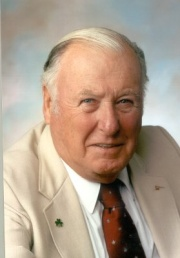
\includegraphics[width=0.22\linewidth]{cooley.jpg}\hspace{2cm}
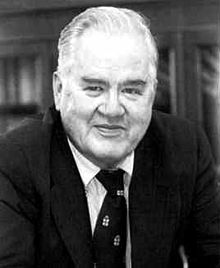
\includegraphics[width=0.25\linewidth]{tukey.jpg}
\caption{\scriptsize{James Cooley \hspace{3.5cm}  John Tukey}}
\end{figure}
\end{frame}

\begin{frame}
\frametitle{FFT Libraries}
\begin{itemize}
\item In python one can use numpy.fft.fft().
\item In MATLAB just need to use fft() or fftw().
\item There are various libraries available in C but probably the most popular one is fftw. The fftw package was developed at MIT by Matteo Frigo and Steven G. Johnson.  
\end{itemize}
\end{frame}

\begin{frame}[fragile] % Need to use the fragile option when verbatim is used in the slide
\frametitle{FFTW in C}
\begin{example}
\begin{verbatim}
#include <fftw3.h>
...
{
fftw_complex *in, *out;
fftw_plan p;
...
in = (fftw_complex*) fftw_malloc(sizeof(fftw_complex) * N);
out = (fftw_complex*) fftw_malloc(sizeof(fftw_complex) * N);
p = fftw_plan_dft_1d(N,in,out,FFTW_FORWARD,FFTW_ESTIMATE);
...
fftw_execute(p);
...
fftw_destroy_plan(p);
fftw_free(in); fftw_free(out);
\end{verbatim}
\end{example}
\end{frame}

%------------------------------------------------




%------------------------------------------------

%\begin{frame}[fragile] % Need to use the fragile option when verbatim is used in the slide
%\frametitle{Citation}
%An example of the \verb|\cite| command to cite within the presentation:\\~

%This statement requires citation \cite{p1}.
%\end{frame}

%------------------------------------------------

\begin{frame}
\frametitle{References}
\begin{enumerate}
\item\url{https://en.wikipedia.org/wiki/Fast_Fourier_transform}
\item\url{https://en.wikipedia.org/wiki/Discrete_Fourier_transform}
\item\url{http://www.fftw.org}
\item\url{https://www.mathworks.com/help/matlab/ref/fft.html}
\item\url{https://docs.scipy.org/doc/numpy/reference/generated/numpy.fft.fft.html}		
\end{enumerate}
\end{frame}

%------------------------------------------------

\begin{frame}
\Huge{\centerline{The End}}
\end{frame}

%----------------------------------------------------------------------------------------

\end{document}